\documentclass[]{article}
\usepackage[a4paper, total={15cm,23cm}]{geometry}
\usepackage{fancyhdr}
\usepackage{graphicx}
\usepackage{amsmath}
\usepackage{amssymb}
\usepackage{xcolor}
\usepackage{cancel}
%opening
\title{PH 222 Activity 2}
\author{Benjamin Bauml}
\date{Winter 2021}
\pagestyle{fancy}
\rhead{PH 222}
\chead{Winter 2021}
\lhead{Activity 2}

%Custom Quotation Command
\newcommand{\excerpt}[1]{\colorbox{lightgray}{\parbox{14.8cm}{#1}} \\}

\begin{document}

\maketitle

\begin{center}
Except for Activity 3, these problems are borrowed/adapted from Chapter 8 of the \textit{Student Workbook} for \textit{Physics for Scientists and Engineers}.
\end{center}
\section*{Activity 1}%7
\excerpt{
The figures are a bird's-eye view of particles on a string moving in horizontal circles on a tabletop. All are moving at the same speed. Rank in order, from largest to smallest, the string tensions $ T_{1} $ to $ T_{4} $
}
\begin{center}
	\includegraphics[scale=0.5]{Circles}
\end{center}
% To reveal the solution, delete "\phantom{\parbox{\textwidth}{" from the beginning, and "}}" from the end.
\phantom{\parbox{\textwidth}{
Order: $ T_{3} > T_{1} = T_{4} > T_{2} $ \\
Explanation: We know that $ T_{1} = \frac{mv^{2}}{r} $ by the nature of centripetal force. Case 2 has a twice the radius, so $ T_{2} = \frac{1}{2} T_{1} $. Case 3 has twice the mass, so $ T_{3} = 2T_{1} $. Case 4 has twice the radius \textit{and} twice the mass, so the two changes cancel each other out. \\
}}

\section*{Activity 2}%13
\excerpt{
A stunt plane does a series of vertical loop the loops at a fairly steady speed. At what point in the circle does the pilot feel the heaviest? Explain. Include a free-body diagram with your explanation.
}
% To reveal the solution, delete "\phantom{\parbox{\textwidth}{" from the beginning, and "}}" from the end.
\phantom{\parbox{\textwidth}{
\begin{center}
	\includegraphics[scale=0.4]{PilotFBDs}
\end{center}
At the bottom, to have a centripetal force that turns the pilot upward in a loop, the normal force on the pilot must exceed the force of gravity upon him. The normal force at the top of the loop works with the force of gravity to turn the pilot toward the ground, so it need not be so large. The pilot feels heaviest at the bottom of the vertical loop, where the normal force on the pilot is greatest. (Note: A weighing scale under the pilot would give a reading equal to the normal force.)
}}

\section*{Activity 3}
\excerpt{
The expression $ \vec{F}_{g} = m\vec{g} $ is an approximation that we use near the Earth's surface. In this problem, we will see how much this approximation is affected by the rotation of the Earth.
}
\excerpt{
(a) Imagine you are in a reference frame where you do not rotate with the Earth, and draw a pictorial representation and free-body diagram for a person (of mass $ m $) standing at the equator. Remember, this person is traveling at some tangential speed $ v_{t} $ at a distance $ R $ from the Earth's center.
}
% To reveal the solution, delete "\phantom{\parbox{\textwidth}{" from the beginning, and "}}" from the end.
\phantom{\parbox{\textwidth}{
\begin{center}
	\includegraphics[scale=0.3]{EarthDiagram}
	\vspace{-35pt}
\end{center}
Note that the need for a centripetal net force suggests that $ F_{g} > n $. \\
}}
\excerpt{
(b) Write an expression for the centripetal force in terms of the forces in your free-body diagram. What should your normal force equal? (Hint: Now you may think in the person's reference frame.)
}
% To reveal the solution, delete "\phantom{\parbox{\textwidth}{" from the beginning, and "}}" from the end.
\phantom{\parbox{\textwidth}{
\[
m\frac{v_{t}^{2}}{R} = F_{c} = F_{net} = F_{g} - n
\]
In the reference frame of the person, approximated gravity pushes down upon him with magnitude $ mg $, and since he is stationary relative to the surface of the Earth, the normal force must counteract this, so $ n = mg $. \\
}}
\excerpt{
(c) The mean radius of the Earth is about $ 6.37\times 10^{6} $ m, and it takes one day for a point on the equator to make one circuit around the globe. What is $ v_{t} $?
}
% To reveal the solution, delete "\phantom{\parbox{\textwidth}{" from the beginning, and "}}" from the end.
\phantom{\parbox{\textwidth}{
The Earth has an equatorial circumference of $ 2\pi R \approx 4.00 \times 10^{7} $ m, so a point which travels this distance in one day must be traveling at
\[
v_{t} = \frac{2\pi\cdot6.37\times 10^{6}\text{ m}}{1\text{ day}} \times \frac{1\text{ day}}{24\text{ h}} \times \frac{1\text{ h}}{60\text{ min}} \times \frac{1\text{ min}}{60\text{ s}} \approx 463 \text{ m/s}
\]
}}
\excerpt{
(d) Using the equation from part (b) Find the gravitational acceleration in the external reference frame.
}
% To reveal the solution, delete "\phantom{\parbox{\textwidth}{" from the beginning, and "}}" from the end.
\phantom{\parbox{\textwidth}{
Let $ g' $ be the gravitational acceleration in the external reference frame. Thus, $ F_{g} = mg' $.
\[
\begin{split}
	m\frac{v_{t}^{2}}{R} & = F_{g} - n \\
	m\frac{v_{t}^{2}}{R} & = mg' - mg \\
	g' & = \frac{v_{t}^{2}}{R} + g \\
	& \approx \frac{(463 \text{ m/s})^{2}}{6.37\times10^{6}} + 9.8\text{ m/s}^{2} \\
	& \approx \frac{(463 \text{ m/s})^{2}}{6.37\times10^{6}} + 9.8\text{ m/s}^{2} \\
	& \approx 9.83 \text{ m/s}^{2}.
\end{split}
\]
The rotation of the Earth lessens the effective gravitational acceleration by about 0.03 m/s$ ^{2} $.
}}

\section*{Activity 4}%15
\excerpt{
It's been proposed that future space stations could create ``artificial gravity'' by rotating around an axis.
}
\excerpt{
(a) How would this work? Explain.
}
% To reveal the solution, delete "\phantom{\parbox{\textwidth}{" from the beginning, and "}}" from the end.
\phantom{\parbox{\textwidth}{
\begin{center}
	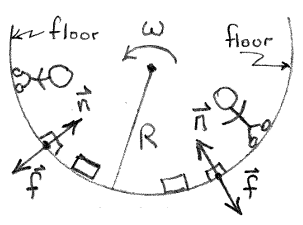
\includegraphics[scale=0.6]{SpaceStation}
\end{center}
People in a rotating station feel a fictitious force ($ \vec{f} $) that ``throws'' them against the outside floor of the station (just as you feel thrown away from the center when your car turns a corner). The fictitious force is opposite the real net force provided by the normal force from the floor. Design the station such that centripetal acceleration $ a_{c} = \omega^{2}R \approx 9.8 $ m/s$ ^{2} $. \\
}}
\excerpt{
(b) Would the artificial gravity be equally effective throughout the space station? If not, where in the space station would the residents want to live and work?
}
% To reveal the solution, delete "\phantom{\parbox{\textwidth}{" from the beginning, and "}}" from the end.
\phantom{\parbox{\textwidth}{
The artificial gravity would not be equally effective throughout the station since the acceleration $ (\omega^{2} r) $ depends on the radial distance $ (r) $ from the center. The residents would want to live on the outside floor where the radius is large enough to give the desired acceleration.
}}

\end{document}